\newpage
\subsection{Caso d'uso UC8 - Interazione Con API non acquistate}
\label{UC8}
\begin{figure}[ht]
	\centering
	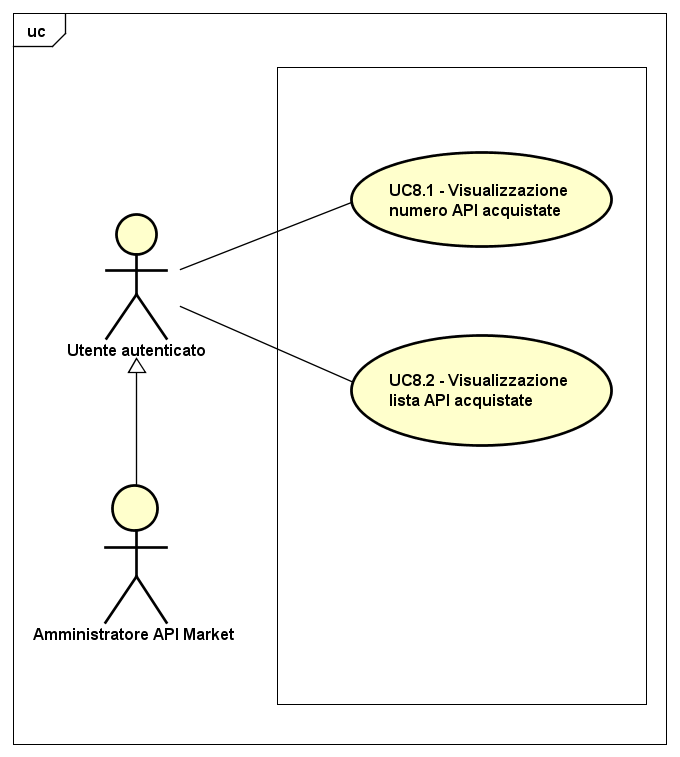
\includegraphics[scale=0.45]{UML/UC8.png}
	\caption{UC8 - Interazione Con API non acquistate}
\end{figure}

\begin{longtable}{ l | p{11cm}}
	\hline
	\rowcolor{Gray}
	\multicolumn{2}{c}{UC8 - Interazione Con API non acquistate}\\
	\hline
	
	 \textbf{Attori} & Utente autenticato  \\
	\textbf{Descrizione} & L'utente puo' interagire con le API non aquistate in vari modi. Visualizza una lista di API e puo' filtrarle, puo' consultarne la documentazione di ognuna, puo' acquistarle \\
	\textbf{Pre-Condizioni} & L'utente e' nella schermata di interazione con le API\\
	\textbf{Post-Condizioni} & L'utente ha scelto l'interazione con le API\\
	\textbf{Scenario Principale} & 
	\begin{enumerate*}[label=(\arabic*.),itemjoin={\newline}]
		\item L'utente puo' cercare una API (UC6)
		\item L'utente puo' cercare una API (UC8.1)
		\item L'utente puo' cercare una API (UC8.2)
	\end{enumerate*}\\
\end{longtable}

